\usepackage{xcolor}
\usepackage{afterpage}
\usepackage{pifont,mdframed}
\usepackage[bottom]{footmisc}
\usepackage{minted}

\createsection{\Grader}{Grader di prova}
\newcommand{\inputfile}{\texttt{stdin}}
\newcommand{\outputfile}{\texttt{stdout}}
\makeatletter
\renewcommand{\this@inputfilename}{\texttt{stdin}}
\renewcommand{\this@outputfilename}{\texttt{stdout}}
\renewcommand{\this@syllabuslevel}{5}
\renewcommand{\this@custdifficulty}{3}
\makeatother

% % % % % % % % % % % % % % % % % % % % % % % % % % % % % % % % % % % % % % % % % % %
% % % % % % % % % % % % % % % % % % % % % % % % % % % % % % % % % % % % % % % % % % %
Durante una sessione di gioco al famosissimo locale \textit{QN32} Andrea, in seguito ad una scommessa di troppo,
si ritrova senza \textit{Soldi}\footnote[1]{Una peculiare valuta internazionale, $1$ \textit{Soldo} $\approx 1.18$€.}.
Nonostante la terribile situazione, si convince che il miglior modo per recuperare il suo capitale sia
ignorare i consigli dei suoi amici e continuare a giocare, ma ad un gioco diverso.
Il gioco da lui scelto è \textit{Pinball 2D}\footnote[2]{Antenato del gioco Toscano "\textit{Calcetto 3D}".}.

\begin{figure}[h]
    \centering
    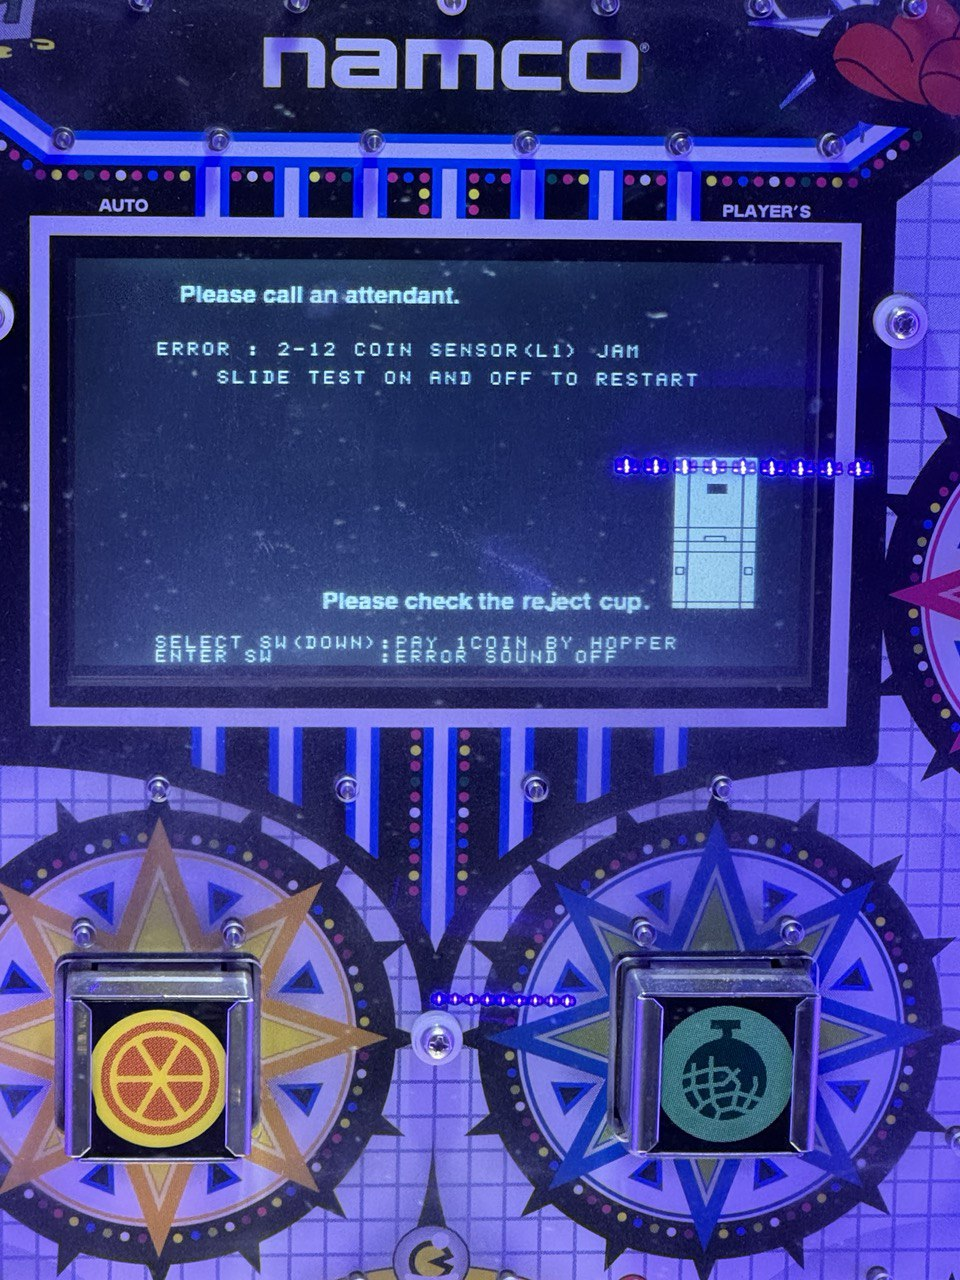
\includegraphics[width=0.4\textwidth]{./broken.jpg}
    \caption{\textit{Pinball 2D}, momenti dopo il disastro.}
\end{figure}

Il gioco funziona così: ci sono $N$ paletti disposti su un piano cartesiano infinito alle coordinate $(x_i, y_i)$, per ogni $i = 0\dots N-1$.
I paletti possono essere alzati o abbassati. L'obiettivo del gioco è scegliere un insieme di paletti da alzare
e formarci un poligono non intrecciato. Al giocatore verranno forniti tanti \textit{Soldi} quanti sono i \textbf{punti a coordinate intere}
contenuti dal poligono, esclusi quelli che appartengono al perimetro della figura.


Nota che scelto un insieme di $K$ paletti da alzare si possono formare$\frac{K!}{2K}$ poligoni.
Sta al giocatore scegliere quello che massimizza i \textit{Soldi} vinti!

Visto l'evidente "\textit{Skill Issue}" di Andrea in geometria, aiutalo a trovare il massimo capitale di \textit{Soldi}
che può vincere! Dato che questo valore può essere enorme, dovrai restituire la risposta \textbf{modulo 1\:000\:000\:007}.

\Implementation

Dovrai sottoporre un unico file, con estensione \texttt{.cpp}.

\begin{warning}
    Tra gli allegati a questo task troverai un template \texttt{pinball.cpp} con un esempio di implementazione.
\end{warning}

Il file di input è composto da $N+1$ righe:
\begin{itemize}
    \item Riga 1: l'intero $N$.
    \item Riga 2 \dots $N+1$: le coordinate $x_i$ e $y_i$.
\end{itemize}

Il file di output è composto da $1$ riga:
\begin{itemize}
    \item Riga 1: la risposta al problema.
\end{itemize}

% % % % % % % % % % % % % % % % % % % % % % % % % % % % % % % % % % % % % % % % % % %
% % % % % % % % % % % % % % % % % % % % % % % % % % % % % % % % % % % % % % % % % % %

\Constraints

\begin{itemize}[nolistsep, itemsep=2mm]
    \item $1 \le N \le 1\:000\:000$.
    \item $-1\:000\:000 \le x_i, y_i \le 1\:000\:000$.
\end{itemize}

% % % % % % % % % % % % % % % % % % % % % % % % % % % % % % % % % % % % % % % % % % %
% % % % % % % % % % % % % % % % % % % % % % % % % % % % % % % % % % % % % % % % % % %

\Scoring

Il tuo programma verrà testato su diversi test case raggruppati in subtask.
Per ottenere il punteggio relativo ad un subtask,
è necessario risolvere correttamente tutti i test che lo compongono.

\IIOTsubtask{0}{1}{Casi d'esempio.}

\IIOTsubtask{30}{1}{Gli insiemi di tutte le $x_i$ e le $y_i$ hanno entrambi cardinalità $2$.}

\IIOTsubtask{50}{3}{$N \le 10$.}

\IIOTsubtask{5}{5}{$-10\:000 \le x_i, y_i \le 10\:000$.}

\IIOTsubtask{15}{5}{Nessuna limitazione aggiuntiva.}


% % % % % % % % % % % % % % % % % % % % % % % % % % % % % % % % % % % % % % % % % % %
% % % % % % % % % % % % % % % % % % % % % % % % % % % % % % % % % % % % % % % % % % %

\Examples

\begin{example}
    \exmpfile{pinball.input0.txt}{pinball.output0.txt}%
    \exmpfile{pinball.input1.txt}{pinball.output1.txt}%
\end{example}

% % % % % % % % % % % % % % % % % % % % % % % % % % % % % % % % % % % % % % % % % % %
% % % % % % % % % % % % % % % % % % % % % % % % % % % % % % % % % % % % % % % % % % %

\Explanation

Nel primo esempio sono evidenziati in blu i paletti, in arancione il perimetro del poligono e in
rosso i punti compresi nella figura.
Con questa configurazione, il giocatore vince $9$ \textit{Soldi} e si può dimostrare che non esiste soluzione migliore.
Il paletto a coordinate $(2,3)$ è abbassato, e viene contato come punto contenuto dal poligono.

\begin{figure}[h]
    \centering
    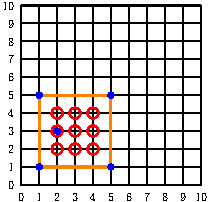
\includegraphics[width=0.4\textwidth]{./asy_examples/example0.pdf}
\end{figure}

Nel secondo caso di esempio, si può dimostrare come il poligono mostrato in figura sia
quello che massimizza i \textit{Soldi} vinti.

\begin{figure}[h]
    \centering
    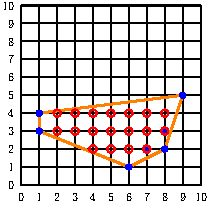
\includegraphics[width=0.4\textwidth]{./asy_examples/example1.pdf}
\end{figure}